%! alt The ellipse x squared plus xy plus y squared equals 360, centred at the origin O, with its long axis along the line y = -x. A and B lie on it with a right angle at O, drawn for OA squared = 288 and OB squared = 480. A right-angle turn of OA changes the sign of s, so the two squared distances are 360 over 1 + s and 360 over 1 - s.
%! after_paragraph 2
%! scale 1/7
% The shared preamble of every Kyuclid figure. pipeline/figures turns these colours into theme-aware paint,
% and refuses any other colour, so draw only with them:
%   figink (lines and labels), figaux (construction lines), figaccent (the object the argument turns on),
%   figtint and figaccenttint (light fills).
\documentclass[border=1.5pt]{standalone}
\usepackage{tkz-euclide}
\definecolor{figink}{RGB}{0,0,0}
\definecolor{figaux}{RGB}{85,85,85}
\definecolor{figaccent}{RGB}{192,57,43}
\definecolor{figtint}{RGB}{221,221,221}
\definecolor{figaccenttint}{RGB}{245,213,208}
% tkz-euclide's defaults draw circles, compasses and marks in 50% grey and fill points with a tint.
\makeatletter
\def\tkz@otherlinecolor{figink}
\def\tkz@euc@circlecolor{figink}
\def\tkz@euc@compasscolor{figink}
\def\tkz@euc@mkcolor{figink}
\def\tkz@mk@fill{figink}
\def\tkz@euc@pointfillcolor{figink}
\makeatother
\tkzSetUpLine[color=figink,line width=.7pt]
\tkzSetUpArc[color=figink,line width=.7pt]
\tkzSetUpCompass[color=figink,line width=.5pt]
\tkzSetUpPoint[color=figink,fill=figink,size=3.1pt]
\tikzset{
  every picture/.style={line cap=round,line join=round,color=figink},
  circle style/.append style={color=figink,line width=.7pt},
  aux/.style={color=figaux,line width=.45pt,dash pattern=on 2.6pt off 2pt},
  key/.style={color=figaccent,line width=1pt},
  mk/.style={color=figink,line width=.5pt},
  lbl/.style={color=figink,inner sep=2.2pt},
  len/.style={color=figink,inner sep=1.5pt,font=\small},
}

\begin{document}
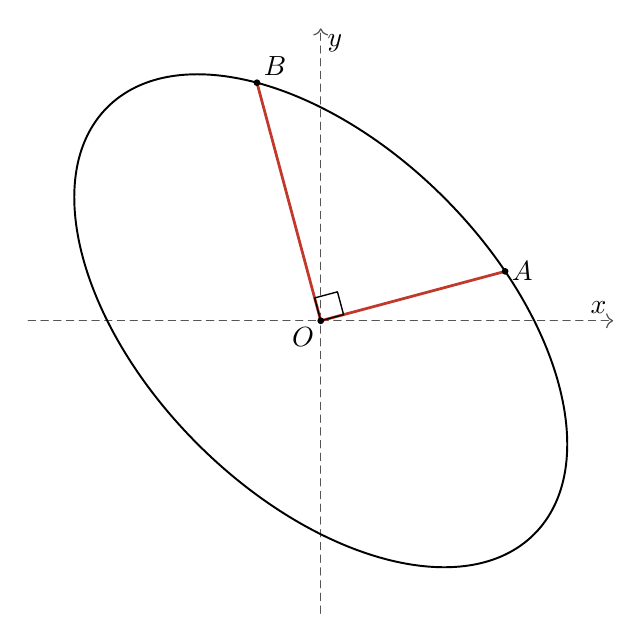
\begin{tikzpicture}
\tkzDefPoint(0.0,0.0){O} %! O = (0, 0)
\tkzDefPoint(2.3417578,0.62747212){A} %! A = polar(O, sqrt(288), 15)
\tkzDefPoint(-0.81006302,3.0231964){B} %! B = polar(O, sqrt(480), 105)
\tkzDefPoint(-3.7142857,0.0){XL} %! XL = (-26, 0)
\tkzDefPoint(3.7142857,0.0){XR} %! XR = (26, 0)
\tkzDefPoint(0.0,-3.7142857){YL} %! YL = (0, -26)
\tkzDefPoint(0.0,3.7142857){YH} %! YH = (0, 26)
\tkzDefPoint(2.7105237,-2.7105237){V} %! V = polar(O, sqrt(720), -45)
\tkzDefPoint(1.5649216,1.5649216){W} %! W = polar(O, sqrt(240), 45)
%! fact equal(x(A)**2 + x(A)*y(A) + y(A)**2, 360)
%! fact equal(x(B)**2 + x(B)*y(B) + y(B)**2, 360)
%! fact equal(x(V)**2 + x(V)*y(V) + y(V)**2, 360)
%! fact equal(x(W)**2 + x(W)*y(W) + y(W)**2, 360)
%! fact angle(A, O, B) == 90
%! fact equal(dist(O, A)**2, 288)
%! fact equal(dist(O, B)**2, 480)
%! fact equal(1/dist(O, A)**2 + 1/dist(O, B)**2, 1/180)
\draw[aux,->] (XL) -- (XR);
\draw[aux,->] (YL) -- (YH);
\draw[rotate=-45,line width=.7pt] (O) ellipse [x radius=3.833260,y radius=2.213133];
\tkzDrawSegments[key](O,A O,B)
\tkzMarkRightAngle[size=.3,mk](A,O,B)
\tkzDrawPoints(O,A,B)
\tkzLabelPoint[right,lbl](A){$A$}
\tkzLabelPoint[above right,lbl](B){$B$}
\tkzLabelPoint[below left,lbl](O){$O$}
\tkzLabelPoint[above left,lbl](XR){$x$}
\tkzLabelPoint[below right,lbl](YH){$y$}
\end{tikzpicture}
\end{document}
